% TODO - FIRST TRY EXPERIMENT WITHOUT STFT

\subsection{Attack Description} % ~ 2.5 to 3 pages (including subsections)
\label{sec:exp:description}

% TODO intro

The following paragraphs give a detailed description of the main steps to realize such an attack. Therefore, we first need to look more precisely at the functional principle of smart light bulbs. Further we have a look at how smooth brightness changes are achieved and how we actually get data out of the received signal.\newline

%write about brightness change frequency, why high sampling frequency is needed, Human eye threshold; mention parts in python program ... 

% TODO ?? talk about Short-time Fourier transform in corresponding section -> To illustrate the temporal change of the frequency spectrum of a signal.

\subsubsection{Controlling Smart Light Bulbs} 
% --> describe components of smart LEDs, how they work, controller communication
Smart light bulbs consist of three main components: (1) a RF~receiver, (2) a processing unit and (3) LEDs and LED~drivers.
The communication with the controller is ensured through the \textit{RF~receiver} and relies on the ZLL~protocol. The received commands are further forwarded to the \textit{processing unit} which interprets the processed signal and controls the LED by modulating the pulse width. The PWM allows the different dimming factors. When sending a brightness change command via the Hue API, this automatically forces the processing unit to generate the corresponding PWM signal. The PWM is sent to the \textit{LED~drivers} which further turn the LEDs on and off at a very fast rate such that those changes in the duty cycle cannot be seen by the human eye. Since Hue comes with 255~brightness~levels which need to be differentiated smoothly, a PWM with a frequency around 20~KHz is used~\cite{Ronen:2016:EFAIDCSL}. 

% TODO: for the following 2 sections to complete need to discuss what we now actually see and used sampling rate, which pics we want to use etc
\subsubsection{Crafting PWM Signal}
% --> describe how fast changes are achieved, frequency output with light sensor, collection of signal with PicoScope
% 10 MS/s = 10 MHz

% TODO fill in concrete values
Since we can no longer craft a custom PWM signal using the Hue~API, we had to get along with the PWM used for dimming.
Thus, our goal was to use close brightness levels and attempt to distinguish them from their PWM profile.

Because of the great amount of brightness levels, we had to measure very small off periods of about 200~ns. This could be done with the described light sensor as well as the PicoScope, since the light sensor's output is around 800~KHz, which we could easily sample at 10~MS/s with our PicoScope.

\subsubsection{Getting Data}
% --> describe analysis of signal
Our primary goal was to distinguish adjacent brightness levels that cannot be distinguished by the human eye.
For this purpose, we performed a Short-Time~Fourier~Transformation~(STFT) to transform the voltage sinusoid obtained from the light sensor into the frequency-over-time domain.

As can be seen in Figure~\ref{fig:plot-140-135}, the difference between brightness levels is clearly visible upon optical inspection of the graph.
For comparison, we found that it took around 10--15 levels of separation for the naked eye to distinguish 2 brightness levels, depending on the absolute brightness.
In the best images, the PWM profiles were clearly recognizable.

However, we had a rather hard time consistently reproducing images.
Distance from the light to the sensor, angle, and variations in external light, in decreasing order, made it harder to clearly distinguish the brightness levels and to choose a starting brightness.
In particular, the square curve tended to become a muddy sinusoid, which we attribute partly to the fact that we perform STFT on the data.
We found that distance between sensor and light had a strong impact on the correct choice of STFT window size and intensity of the brightness levels between which we switch, with increasing distance requiring more energy and/or a smaller window.

\begin{figure}[h]
	\centering
	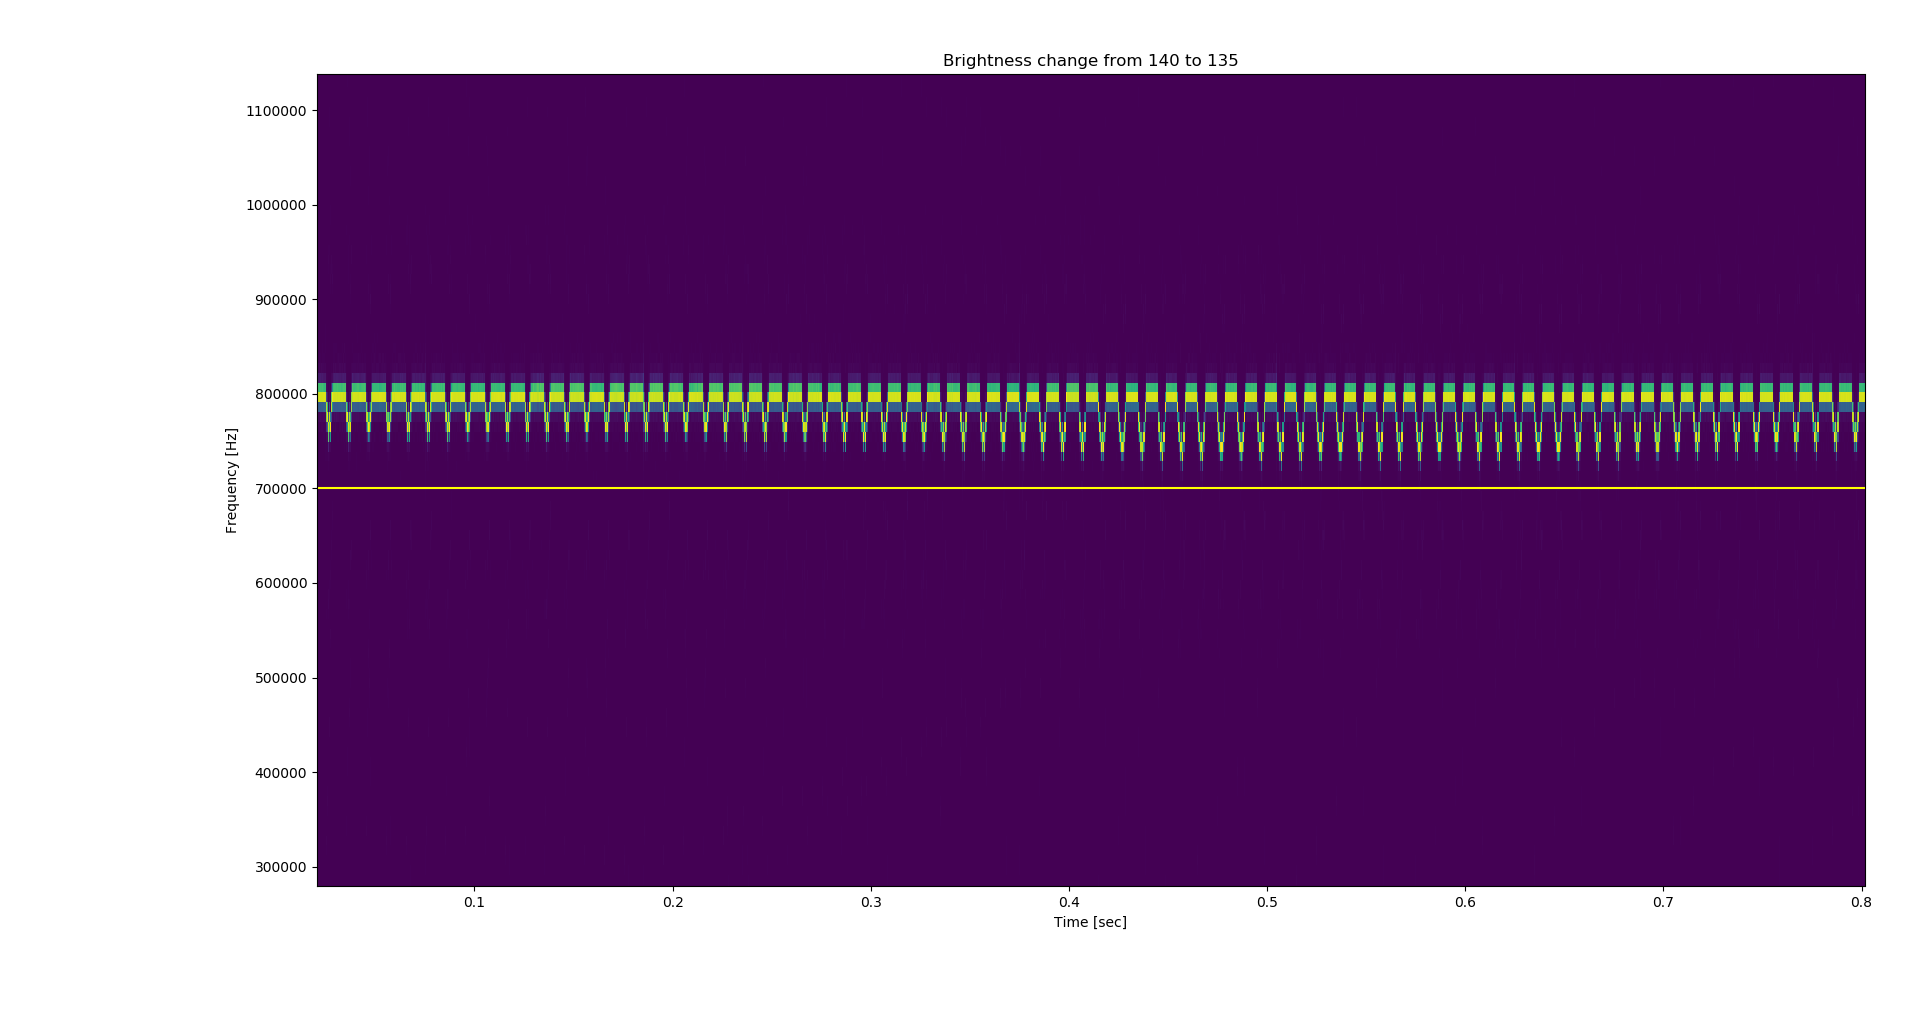
\includegraphics[width=14cm]{img/Plot_140_135.png}
	\caption{Brightness change from levels 140 to 135 (and back) sampled at 10 MS/s. Note the smooth fading.}
	\label{fig:plot-140-135}
\end{figure}

We were not able to robustly automatically distinguish brightness levels, but that may be because we spent most of our time trying to do that with the Fourier-transformed data when it may have been better to analyze the sinusoid from the light sensor directly.
In any case, this is a solvable signal processing problem and more a question of time.

With that done, the next step would be to select brightness levels for 0 and 1, and maybe a third in between the two to be used as delimiter and reduce the need for synchronization.
All that would then be left to do is to apply a suitable channel coding to the data, send appropriate brightness commands to the light, write out the recognized 0s and 1s, and decode the data.
